\documentclass[11pt, a4paper]{book}

\usepackage[a4paper, left=1.27cm,top=1.27cm,right =1.27cm, bottom = 1.4cm]{geometry}
%\setlength{\parindent}{0cm}

\usepackage[dutch]{babel}
\usepackage{mathtools}
\usepackage{upgreek}
\usepackage{amsfonts}


\usepackage{graphicx}
\graphicspath{{figures/}}

\begin{document}
    
    \tableofcontents

    \chapter{Krachten, momenten, spanningne en rekken}

    \section{STATICA EN EVENWICHT VAN CONSTRUCTIES}

        \subsection{Types ondersteuningen}

            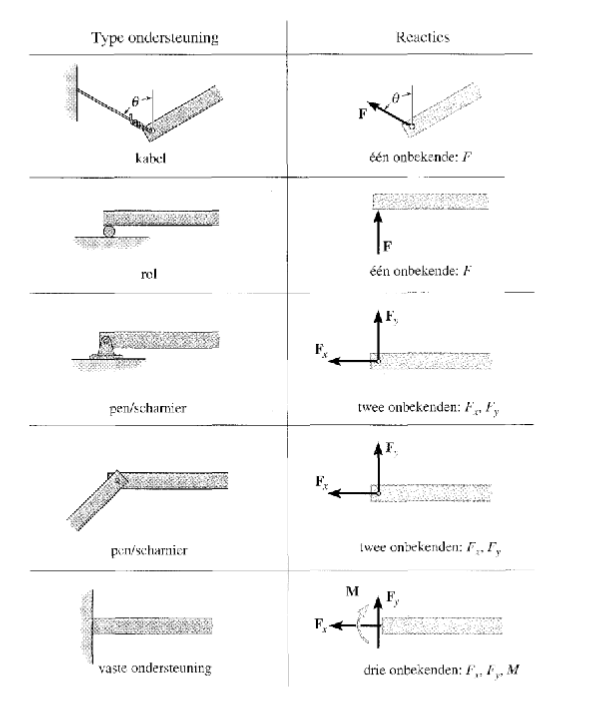
\includegraphics[scale=0.5]{ondersteuningen.png}

        \subsection{Evenwicht van een constructie}

            \begin{align*}
                &\sum\mathbf{F} = 0\\
                &\sum\mathbf{M}_O = 0\\
            \end{align*}
    
    \section{INTUÏtIEF BEGRIP VAN SPANNINGEN EN REKKEN}

        \begin{align*}
            &\upsigma = \frac{F}{A_0}\\
            &\upvarepsilon = \frac{\Delta L}{L_0}\\
            &\upsigma = E\cdot \upvarepsilon
        \end{align*}

    \section{SPANNINGEN}
        
        \subsection{Definitie}

            De spanningsvector
            \begin{equation}
                \vec{\upphi}^{(n)} = \lim_{\Delta A \rightarrow 0} \frac{\Delta F}{\Delta A}
                \label{spanningsvector}
            \end{equation}
            De normaalspanning
            \begin{equation}
                \upsigma = \lim_{\Delta A \rightarrow 0} \frac{\Delta F_n}{\Delta A}
                \label{normaalspanning}
            \end{equation}
            De schuifspanning
            \begin{equation}
                \uptau = \lim_{\Delta A \rightarrow 0} \frac{\Delta F_t}{\Delta A}
                \label{schuifspanning}
            \end{equation}
            De spanningstensor
            \begin{equation}
                [\sigma] = \left[\begin{matrix}
                    \upsigma_{xx} & \uptau_{xy} & \uptau_{xz} \\
                    \uptau_{yx} & \upsigma_{yy} & \uptau_{yz} \\
                    \uptau_{zx} & \uptau_{zy} & \upsigma_{zz}
                \end{matrix}\right]
                \label{spanningstensor}
            \end{equation}

        \subsection{Verband tussen spanningsvector $\vec{\upphi}^{(n)}$ en spanningstensor $[\upsigma]$}
            
            Het verband tussen de spanningsvector en spanningstensor
            \begin{equation}
                \upsigma_{ij}\cdot n_i = \upphi_j^{(n)} \;\;\; (i,j=x,y,z)
                \label{spannigsvector_tensor}
            \end{equation}

        \subsection{Vergelijkingen van het evenwicht}

            De vergelijkingen van het evenwicht
            \begin{align}
                &\frac{\partial \upsigma_{xx}}{\partial x} + \frac{\partial \uptau_{yx}}{\partial y} + \frac{\partial \uptau_{zx}}{\partial z} + F_x = 0\nonumber\\
                &\frac{\partial \uptau_{xy}}{\partial x} + \frac{\partial \upsigma_{yy}}{\partial y} + \frac{\partial \uptau_{zy}}{\partial z} + F_y = 0 \\
                &\frac{\partial \uptau_{xz}}{\partial x} + \frac{\partial \uptau_{yz}}{\partial y} + \frac{\partial \upsigma_{zz}}{\partial z} + F_z = 0\nonumber\\
                \label{vergelijkingen_van_het_evenwicht}
            \end{align}
            Wet van de wederkerigheid der schuifspanningen
            \begin{align}
                &\uptau_{xy} = \uptau_{yx}\\
                &\uptau_{xz} = \uptau_{zx}\\
                &\uptau_{yz} = \uptau_{zy}\\
            \end{align}

        \subsection{Transformatie van coördinaten en hoofdrichtingen}

            \begin{equation}
                [\upsigma'] = [a]\cdot[\upsigma)\cdot[a]^{\top}
                \label{spanningstransformatie}
            \end{equation}
            met
            \begin{equation}
                a_{rk} = \vec{e}'_r\cdot\vec{e}_k \;\;\; r,k=x,y,z
                \label{Transformatiematrixelementen}
            \end{equation}
            
        \subsection{Kromlijnige coördinaten}
            
            \subsubsection{Cilindercoördinaten}

                De spanningstensor
                \begin{equation}
                    [\upsigma] = \left[\begin{matrix}
                        \upsigma_{rr} & \uptau_{x\theta} & \uptau_{rz} \\
                        \uptau_{r\theta} & \upsigma_{\theta \theta} & \uptau_{\theta z} \\
                        \uptau_{rz} & \uptau_{\theta z} & \upsigma_{zz}
                    \end{matrix}\right]
                \end{equation}

    \section{Rekken}

        \subsection{Eendimensionale lengteverandering}            
    \chapter{Structureel gedrag}

    \section{GEOMETRISCHE EIGENSCHAPPEN VAN DE DWARSDOORSNEDE}

        \subsection{Opstellen vergelijkingen}

            Oppervlakte van de dwarsdoorsnede
            \begin{equation}
                A=\int\int dy'dz'
            \end{equation}
            Statisch moment om de $y'$-as
            \begin{equation}
                S_{y'} = \int\int z'dy'dz'
            \end{equation}
            Statisch moment om de $z'$-as
            \begin{equation}
                S_{z'} = \int\int y'dy'dz'
            \end{equation}
            Ligging zwaartepunt
            \begin{align}
                y'_o&=\frac{S_{z'}}{A}\nonumber\\
                z'_o&=\frac{S_{y'}}{A}\nonumber\\
            \end{align}
            Traagheidsmomenten van de doorsnede
            \begin{align}
                I_{yy} &= \int\int z^2dydz\nonumber\\
                I_{zz} &= \int\int y^2dydz\nonumber\\
                I_{yz} &= -\int\int yzdydz\nonumber\\
            \end{align}
            Stelling van Steiner (parallel axis theorem)
            \begin{align}
                I_{y'y'} &= I_{yy} + A\cdot(z'_o)^2\nonumber\\
                I_{z'z'} &= I_{zz} + A\cdot(z'_o)^2\nonumber\\
                I_{y'z'} &= I_{yz} - A\cdot y'_o\cdot z'_o\nonumber\\
            \end{align}
            Rotatie van het assenstelsel
            \begin{align}
                I_{y'y'} &= \cos^2\alpha\cdot I_{yy}+\sin^2\alpha\cdot I_{zz} + 2\sin\alpha\cos\alpha\cdot I_{yz}\nonumber\\
                I_{z'z'} &= \sin^2\alpha\cdot I_{yy}+\cos^2\alpha\cdot I_{zz} - 2\sin\alpha\cos\alpha\cdot I_{yz}\nonumber\\
                I_{y'z'} &= -\sin\alpha\cos\alpha\cdot I_{yy} + \sin\alpha\cos\alpha\cdot I_{zz} + \left(\cos^2\alpha - \sin^2\alpha\right)\cdot I_{yz}\nonumber
            \end{align}
            Voor de hoofdtraagheidsmomenten geldt
            \begin{equation}
                \tan 2\alpha = \frac{2I_{yz}}{I_{yy} - I_{zz}}
            \end{equation}
        
        \subsection{Praktische berekening}

            \begin{center}
                \includegraphics[scale=0.525]{tm_t1.png}

                \includegraphics[scale=0.5]{tm_t2.png}

                \includegraphics[scale=0.5]{tm_t3.png}
            \end{center}
            \pagebreak
            \begin{center}
                \includegraphics[scale=0.5]{kenmerken.png}
            \end{center}
            met de weerstandsmomenten gedefinieerd als
            \begin{align}
                W_{y} &= \frac{2\cdot I_{yy}}{h}\nonumber\\
                W_{z} &= \frac{2\cdot I_{zz}}{b}\nonumber
            \end{align}
        
    \section{NORMAALKRACHT, BUIGEND MOMENT EN DWARSKRACHT}

        \subsection{Verband tussen q, V en M}

            \begin{align}
                q &= \frac{-dV}{dx}\nonumber\\
                V &= \frac{dM}{dx}\nonumber\\
                q &= \frac{-d^2M}{dx^2}
            \end{align}

        \subsection{Enkele referentiegevallen}
            
            \subsubsection{Ingeklemde balk met puntlast}

                \begin{center}
                    \includegraphics[scale=0.5]{ingeklemde_balk_met_puntlast.png}
                \end{center}

                \begin{align}
                    V &= F\nonumber\\
                    M &= -F\cdot\left(L-x\right)\nonumber
                \end{align}

            \subsubsection{Ingeklemde balk met verdeelde belasting}

                \begin{center}
                    \includegraphics[scale=0.5]{ingeklemde_balk_met_verdeelde_belasting.png}
                \end{center}

                \begin{align}
                    V &= q\cdot\left(L-x\right)\nonumber\\
                    M &= \frac{-q\cdot\left(L-x\right)^2}{2}\nonumber
                \end{align}

            \subsubsection{Balk op twee steunpunten met puntlast}

                \begin{center}
                    \includegraphics[scale=0.5]{balk_op_twee_steunpunten_met_puntlast.png}
                \end{center}
                
                \begin{align}
                    V &= \left\lbrace\begin{matrix}
                        \frac{F\cdot\left(L-a\right)}{L}\;\;\; , x < a\\
                        \frac{-F\cdot a}{L}\;\;\; , x > a\\
                    \end{matrix}\right.\nonumber\\
                    M &= \left\lbrace\begin{matrix}
                        \frac{F\cdot x\cdot\left(L-a\right)}{L}\;\;\; , x < a\\
                        \frac{F\cdot a\cdot\left(L-x\right)}{L}\;\;\; , x > a\\
                    \end{matrix}\right.\nonumber
                \end{align}

            \subsubsection{Balk op twee steunpunten met verdeelde belasting}

                \begin{center}
                    \includegraphics[scale=0.5]{balk_op_twee_steunpunten_met_verdeelde_belasting.png}
                \end{center}

                \begin{align}
                    V &= q\cdot\left(\frac{L}{2}-x\right)\nonumber\\
                    M &= \frac{q\cdot x \cdot \left(L-x\right)}{2}\nonumber
                \end{align}
        
    \section{VERBAND TUSSEN SNEDEKRACHTEN EN SPANNINGEN}

        \subsection{Spanningen t.g.v. normaalkracht N}

            De spanning t.g.v. de normaalkracht N
            \begin{equation}
                \upsigma_{xx} = \frac{N}{A}
            \end{equation}
            en de bijhorende rek
            \begin{equation}
                \varepsilon_{xx} = \frac{N}{E\cdot A}
            \end{equation}

        \subsection{Spanningen t.g.v. buigend moment M}

            \begin{equation}
                \upsigma_{xx} = \frac{M\cdot z}{I_{yy}}
            \end{equation}
            Kromtestraal
            \begin{equation}
                \frac{1}{R} = \frac{-M}{E\cdot I_{yy}}
            \end{equation}

        \subsection{Spanningen t.g.v. dwarskracht V}

            Formule van Jourawski
            \begin{equation}
                \uptau_{xz}(z) = \frac{V}{I_{yy}}\cdot\frac{S_{y}(z)}{[y_2(z)-y_1(z)]}
            \end{equation}

            \begin{center}
                \includegraphics[scale=0.5]{spanningen_door_MV.png}
            \end{center}

    \section{VERPLAATSINGEN}

        \subsection{Verplaatsingen t.g.v. de normaalkracht N}

            \begin{equation}
                \Delta L = \int_0^L\frac{N}{A\cdot E}dx
            \end{equation}

        \subsection{Verplaatsingen t.g.v. het buigend moment M}

            \begin{equation}
                \frac{d^2u}{dx^2} = \frac{-M}{E\cdot I_{yy}}
            \end{equation}

            \begin{equation}
                q = \frac{-dV}{dx} = \frac{-d^2M}{dx^2} = -EI_{yy}\frac{d^3\alpha}{dx^3} = EI_{yy}\frac{d^4u}{dx^4}
            \end{equation}

            \subsubsection{Ingeklemde balk met puntlast}

                \begin{equation}
                    u(x) = \frac{F}{E\cdot I_{yy}}\cdot\left(L\cdot\frac{x^2}{2}-\frac{x^3}{6}\right)
                \end{equation}

            \subsubsection{Ingeklemde balk met verdeelde belasting}

                \begin{equation}
                    u(x) = \frac{q}{E\cdot I_{yy}}\cdot\left[\frac{(L-x)^4}{24}+\frac{L^3}{6}\cdot x-\frac{L^4}{24}\right]
                \end{equation}

            \subsubsection{Balk op twee steunpunten met puntlast}

                \begin{equation}
                    u(x) = \left\lbrace\begin{matrix}
                        \frac{F}{E\cdot I_{yy}}\cdot\left[-\frac{(L-a)}{L}\cdot\frac{x^3}{6}+\frac{a\cdot (L-a)\cdot(2L-*a)}{6L}\cdot x\right]\;\;\; , x < a\\
                        \frac{F}{E\cdot I_{yy}}\cdot\left[-\frac{a\cdot(L-x)^3}{6L}-\frac{a\cdot(L-a)\cdot(L+a)}{6L}\cdot x + \frac{a\cdot (L-a)\cdot (L+a)}{6}\right]\;\;\; , x > a\\
                    \end{matrix}\right.
                \end{equation}

            \subsubsection{Balk op twee steunpunten met verdeelde belasting}

                \begin{equation}
                    u(x) = \frac{q}{E\cdot I_{yy}}\cdot\left[\frac{1}{24}\cdot x^4 - \frac{L}{12}\cdot x^3 + \frac{L^3}{24}\cdot x\right]
                \end{equation}

    \section{SINGULARITEITSFUNCTIES}

        Voor de verdeelde belasting $q(x)$
        \begin{equation}
            \forall n\in \mathbb{N}: \:\:\: \langle x-a\rangle^n = \left|\begin{matrix}
                0 \:\:\:, x<a\\
                (x-a)^n \:\:\:, x>a
            \end{matrix}\right.
        \end{equation}
        met volgende regels
        \begin{align}
            \frac{d}{dx}\langle x-a\rangle^n = n\cdot\langle x-a\rangle^{n-1}\nonumber\\
            \int\langle x-a\rangle^ndx = \frac{\langle x-a\rangle^{n+1}}{n+1} + C
        \end{align}
        En voor geconcentreerde puntlasten $F$ of koppes $K$
        \begin{align}
            q &= F\cdot\langle x-a\rangle^{-1} = \left|\begin{matrix}
                0 \:\:\:, x<a\\
                F \:\:\:, x>a
            \end{matrix}\right.\nonumber\\
            q &= K\cdot\langle x-a\rangle^{-2} = \left|\begin{matrix}
                0 \:\:\:, x<a\\
                K \:\:\:, x>a
            \end{matrix}\right.
        \end{align}
        met rekenregels $\forall n \in \mathbb{N}$
        \begin{align}
            \frac{d}{dx}\langle x-a\rangle^{-n} = n\cdot\langle x-a\rangle^{-n-1}\nonumber\\
            \int\langle x-a\rangle^{-n}dx = \frac{\langle x-a\rangle^{n+1}}{-n+1}
        \end{align}

    \section{INVLOED VAN DE KEUZE VAN HET ASSENSTELSEL}

        \begin{center}
            \includegraphics[scale=1]{keuze_assenstelsel.png}
        \end{center}

        

            
    \chapter{Tweedimensionale problemen}

\end{document}